%%%%%%%%%%%%%%%%%%%%%%%%%%%%%%%%%%%%%%%%%%%
%
% From a template maintained at https://github.com/jamesrobertlloyd/cbl-tikz-poster
%
% Code near the top should be fairly standard and not need to be changed
%  - except for the document class
% Code lower down is more likely to be customised
%
%%%%%%%%%%%%%%%%%%%%%%%%%%%%%%%%%%%%%%%%%%%

%%%%%%%%%%%%%%%%%%%%%%%%%%%%%%%%%%%%%%%%%%%
%
% Document class
%
% Change this if you want a different size / orientation poster etc
%
%%%%%%%%%%%%%%%%%%%%%%%%%%%%%%%%%%%%%%%%%%%

\documentclass[landscape,a0b,final,a4resizeable]{a0poster}
%\documentclass[portrait,a0b,final,a4resizeable]{a0poster}

%%%%%%%%%%%%%%%%%%%%%%%%%%%%%%%%%%%%%%%%%%%
%
% 'Basic' packages
%
% TODO - Almost certainly some are unnecessary - feel free to remove nonstandard
% packages if you think it is a good idea not to always have them
%
%%%%%%%%%%%%%%%%%%%%%%%%%%%%%%%%%%%%%%%%%%%

\usepackage{multicol}
\usepackage{color}
\usepackage{shadow}
\usepackage{morefloats}
\usepackage{cite}
\usepackage[pdftex]{graphicx}
\usepackage{rotating}
\usepackage{amsmath, amsthm, amssymb, bm}
\usepackage{array}
\usepackage{nth}
\usepackage[square,numbers]{natbib}
\usepackage{booktabs}
\usepackage[table,xcdraw]{xcolor}
\usepackage{wrapfig}

%%%%%%%%%%%%%%%%%%%%%%%%%%%%%%%%%%%%%%%%%%%
%
% TIKZ packages and common definitions
%
% Add extra things as per your tikz needs
%
%%%%%%%%%%%%%%%%%%%%%%%%%%%%%%%%%%%%%%%%%%%

\usepackage{picins}
\usepackage{tikz}
\usetikzlibrary{shapes.geometric,arrows,chains,matrix,positioning,scopes,calc}
\tikzstyle{mybox} = [draw=white, rectangle]

%%%%%%%%%%%%%%%%%%%%%%%%%%%%%%%%%%%%%%%%%%%
%
% myfig
%
% \myfig - replacement for \figure
% necessary, since in multicol-environment 
% \figure won't work        
%                 
%%%%%%%%%%%%%%%%%%%%%%%%%%%%%%%%%%%%%%%%%%%

\newcommand{\myfig}[3][0]{
\begin{center}
  \vspace{1.5cm}
  \includegraphics[width=#3\hsize,angle=#1]{#2}
  \nobreak\medskip
\end{center}}

%%%%%%%%%%%%%%%%%%%%%%%%%%%%%%%%%%%%%%%%%%%
%
% mycaption                
%
% \mycaption - replacement for \caption
% necessary, since in multicol-environment \figure and
% therefore \caption won't work
%
%%%%%%%%%%%%%%%%%%%%%%%%%%%%%%%%%%%%%%%%%%%

%\newcounter{figure}
\setcounter{figure}{1}
\newcommand{\mycaption}[1]{
  \vspace{0.5cm}
  \begin{quote}
    {{\sc Figure} \arabic{figure}: #1}
  \end{quote}
  \vspace{1cm}
  \stepcounter{figure}
}

%%%%%%%%%%%%%%%%%%%%%%%%%%%%%%%%%%%%%%%%%%%
%
% Some standard colours
%
%%%%%%%%%%%%%%%%%%%%%%%%%%%%%%%%%%%%%%%%%%%

\definecolor{camlightblue}{rgb}{0.601 , 0.8, 1}
\definecolor{camdarkblue}{rgb}{0, 0.203, 0.402}
\definecolor{camred}{rgb}{1, 0.203, 0}
\definecolor{camyellow}{rgb}{1, 0.8, 0}
\definecolor{lightblue}{rgb}{0, 0, 0.80}
\definecolor{white}{rgb}{1, 1, 1}
\definecolor{whiteblue}{rgb}{0.80, 0.80, 1}

%%%%%%%%%%%%%%%%%%%%%%%%%%%%%%%%%%%%%%%%%%%
%
% Some look and feel definitions
%
%%%%%%%%%%%%%%%%%%%%%%%%%%%%%%%%%%%%%%%%%%%

\setlength{\columnsep}{0.03\textwidth}
\setlength{\columnseprule}{0.0018\textwidth}
\setlength{\parindent}{0.0cm}

%%%%%%%%%%%%%%%%%%%%%%%%%%%%%%%%%%%%%%%%%%%
%
% \mysection - replacement for \section*
% 
% Puts a pretty box around some text
% TODO - any other thoughts for what this box should look like
%
%%%%%%%%%%%%%%%%%%%%%%%%%%%%%%%%%%%%%%%%%%%

\tikzstyle{mysection} = [rectangle, 
									draw=none, 
									shade, 
									outer color=camlightblue!30,
									inner color=camlightblue!30,
									text width=0.965\columnwidth,
									text centered,
									rounded corners=20pt,
									minimum height=0.11\columnwidth]

\newcommand{\mysection}[1]
{
\begin{center}
  \begin{tikzpicture}
    \node[mysection] {\sffamily\bfseries\LARGE#1};
  \end{tikzpicture}
\end{center}
}

%%%%%%%%%%%%%%%%%%%%%%%%%%%%%%%%%%%%%%%%%%%
%
% Set the font
%
% TODO - Not sure what a canonical choice is - feel free to modify
%
%%%%%%%%%%%%%%%%%%%%%%%%%%%%%%%%%%%%%%%%%%%

\renewcommand{\familydefault}{cmss}
\sffamily

%%%%%%%%%%%%%%%%%%%%%%%%%%%%%%%%%%%%%%%%%%%
%
% Poster environment
%
% Centres everything and can be used to define the width of the content
%
%%%%%%%%%%%%%%%%%%%%%%%%%%%%%%%%%%%%%%%%%%%

\newenvironment{poster}{
  \begin{center}
  \begin{minipage}[c]{0.96\textwidth}
}{
  \end{minipage} 
  \end{center}
}

%%%%%%%%%%%%%%%%%%%%%%%%%%%%%%%%%%%%%%%%%%%
%
% This is probably a good place to put content specific packages and definitions
%
%%%%%%%%%%%%%%%%%%%%%%%%%%%%%%%%%%%%%%%%%%%

%%%%%%%%%%%%%%%%%%%%%%%%%%%%%%%%%%%%%%%%%%%
%
% The document environment starts here
%
%%%%%%%%%%%%%%%%%%%%%%%%%%%%%%%%%%%%%%%%%%%

\begin{document}

%%%%%%%%%%%%%%%%%%%%%%%%%%%%%%%%%%%%%%%%%%%
%
% Begin the poster environment - centres things and potentially changes the width
%
%%%%%%%%%%%%%%%%%%%%%%%%%%%%%%%%%%%%%%%%%%%

\begin{poster}

%%%%%%%%%%%%%%%%%%%%%%%%%%%%%%%%%%%%%%%%%%%
%
% Potentially add some space at the top of the poster
%
%%%%%%%%%%%%%%%%%%%%%%%%%%%%%%%%%%%%%%%%%%%

\vspace{0\baselineskip}

%%%%%%%%%%%%%%%%%%%%%%%%%%%%%%%%%%%%%%%%%%%
%
% Draw the header as a TIKZ picture
%
% Using TIKZ to allow for easy alignment
%
%%%%%%%%%%%%%%%%%%%%%%%%%%%%%%%%%%%%%%%%%%%

\begin{center}
\begin{tikzpicture}[x=0.5\textwidth]
    % Dummy nodes at edges for spacing
    % TODO - a better way?
    \node at (+1, 0) {};    
    \node at (-1, 0) {};
    % Set the size of the badges
    \def \badgeheight {0.08\textwidth}
    % Title text
    \node[inner sep=0,text width=0.5\textwidth,text centered,font=\Huge] (Title) at (0,0) 
    {
        {\sffamily\Huge \textbf{Geomagnetic activity, Space Weather and Machine Learning}}\\
        {\sffamily\huge Mandar Chandorkar, Enrico Camporeale\textsuperscript{1}}\\
        \vspace{-0.3\baselineskip}
        {\sffamily\large 1: Multiscale Dynamics, Centrum Wiskunde Informatica}
    };
    % Cambridge badge
    \node [mybox] (CWI Logo) at (-0.9, 0) {
        
\includegraphics[height=\badgeheight]{cwi-logo.png}
    };
    % CBL badge
    \node [mybox] (Inria logo) at (+0.8, 0) {
        
\includegraphics[height=\badgeheight]{inria-logo.jpg}
    };
\end{tikzpicture}
\end{center}

%%%%%%%%%%%%%%%%%%%%%%%%%%%%%%%%%%%%%%%%%%%
%
% Spacing between title and main body
%
%%%%%%%%%%%%%%%%%%%%%%%%%%%%%%%%%%%%%%%%%%%

\vspace{3\baselineskip}

%%%%%%%%%%%%%%%%%%%%%%%%%%%%%%%%%%%%%%%%%%%
%
% Columns environment
%
%%%%%%%%%%%%%%%%%%%%%%%%%%%%%%%%%%%%%%%%%%%

\begin{multicols}{3}

%%%%%%%%%%%%%%%%%%%%%%%%%%%%%%%%%%%%%%%%%%%
%
% Start of content
%
%%%%%%%%%%%%%%%%%%%%%%%%%%%%%%%%%%%%%%%%%%%

\large

\mysection{Space Weather}

\vspace{\baselineskip}

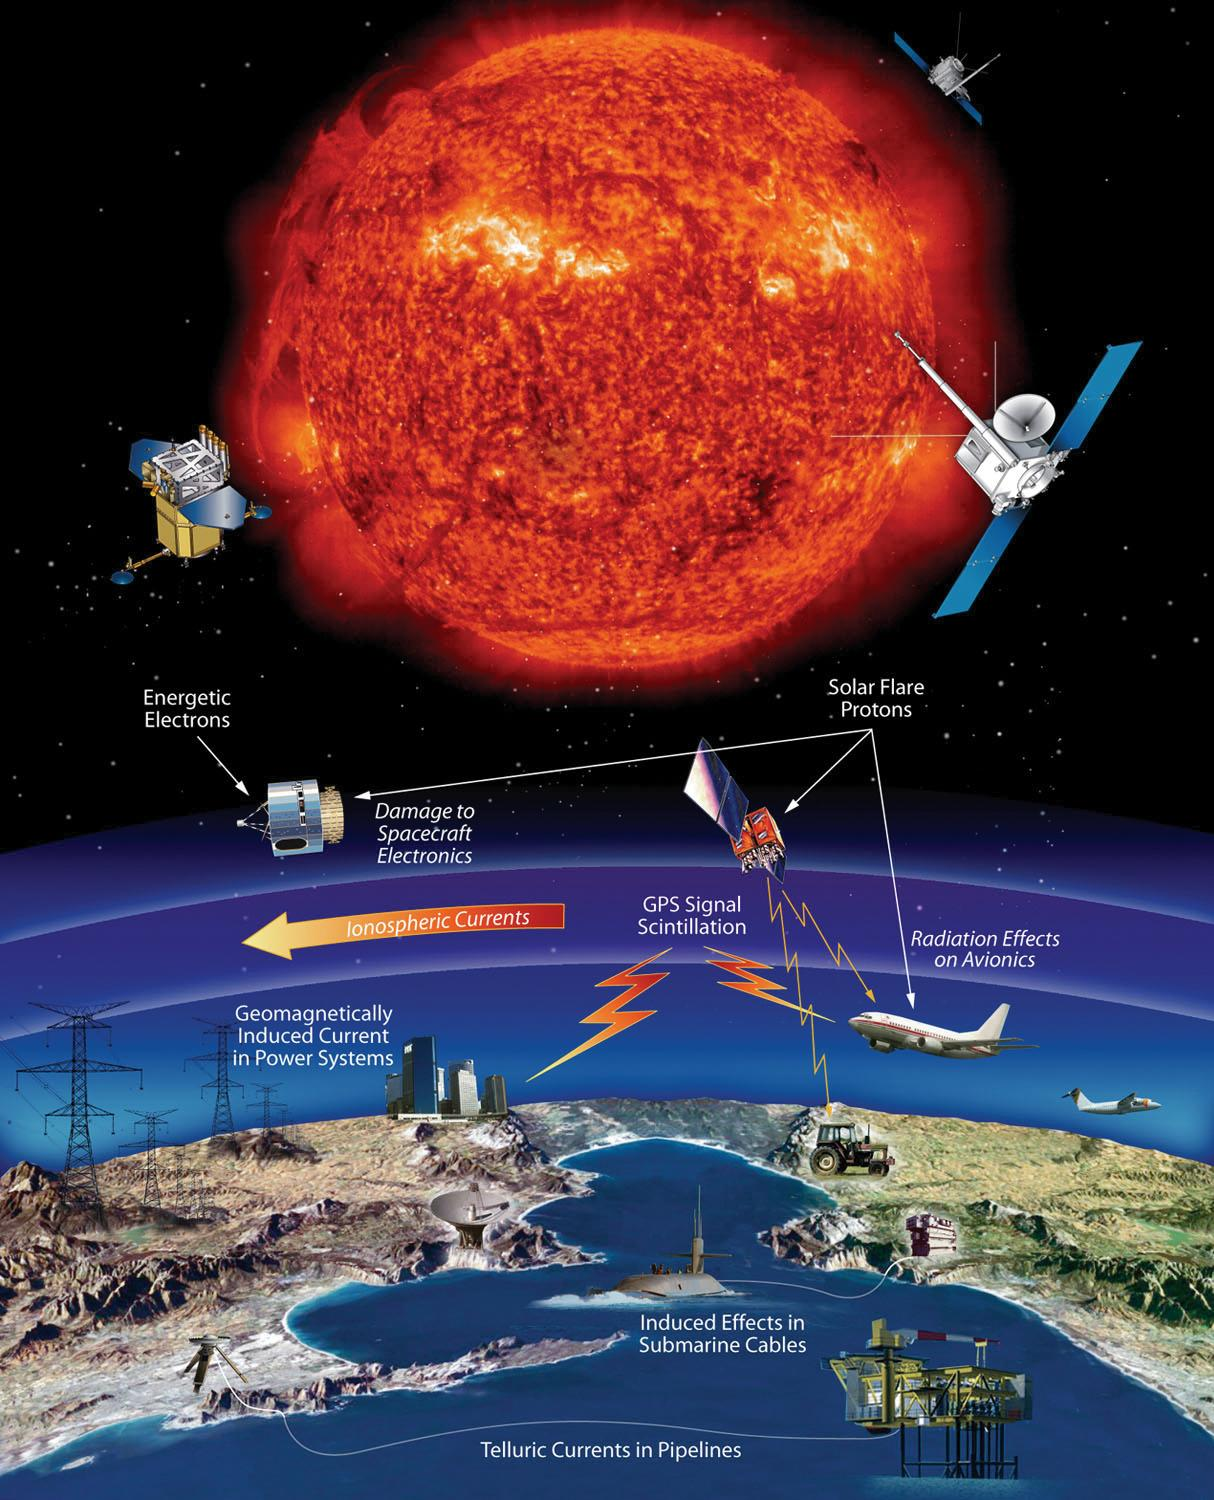
\includegraphics[height=40cm]{nasa-space-weather}

\vspace{\baselineskip}

Space weather is a branch of space physics concerned with the time varying conditions within the Solar System, including the solar wind, emphasizing the space surrounding the Earth, including conditions in the magnetosphere and ionosphere. 

\begin{itemize}
\item The sun is the main driver of space weather. Bursts of plasma from the sun's atmosphere called coronal mass ejections (CME) together with sudden bursts of radiation, all cause space weather effects here on Earth.

\item Coronal Mass Ejections (CMEs) can cause Geomagnetic Storms at Earth and induce extra currents in the ground that can affect power grid operations.

\item Geomagnetic storms can also modify the signal from radio navigation systems (GPS and GNSS) causing degraded accuracy and produce aurora. 
\end{itemize}

\vspace{\baselineskip}

\mysection{Geomagnetic Activity and Indexes}

\vspace{\baselineskip}

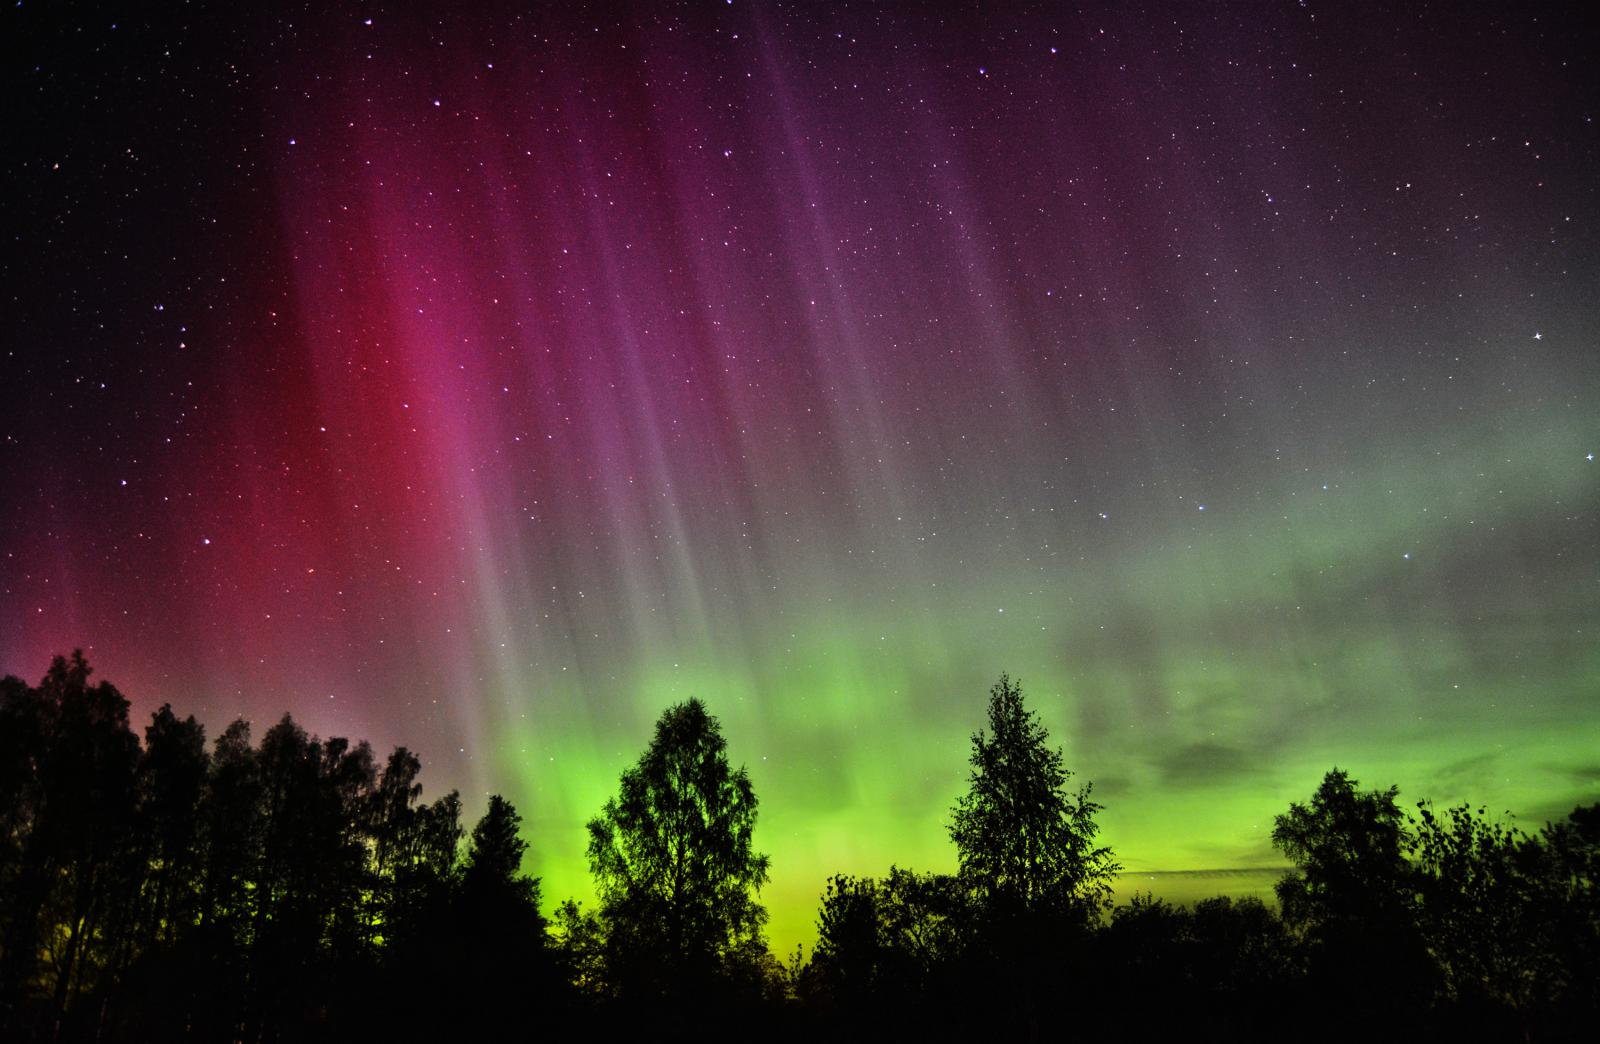
\includegraphics[height=15cm]{aurora}

\vspace{\baselineskip}

Due to the complex nature of the governing dynamics of geo-magnetic response to driving forces (solar wind), it is useful to use representative indexes to record and predict activity of the magnetosphere.


% \vspace{\baselineskip}

%The table below summarizes some important activity indexes which can be considered as a proxy measurement of the geomagnetic response of the Earth towards space weather drivers.

%\vspace{\baselineskip}
%
\vspace{\baselineskip}

\setlength{\arrayrulewidth}{1mm}
\setlength{\tabcolsep}{18pt}
\renewcommand{\arraystretch}{2.5}
 
{\rowcolors{2}{green!80!yellow!50}{green!70!yellow!40}
\begin{tabular}{ |p{2cm}|p{12cm}|p{4cm}|p{6cm}|  }
\hline
Name & Significance & Frequency & Values \\
\hline
Kp   & Global geomagnetic storm index and is based on 3 hour measurements of the K-indices, for a given value, for each of the past days & 3 hours & 0-9          \\
Dst  & Average ring current around magnetic equator & hourly & Real Number  \\
AE   & The AE index is derived from geomagnetic variations in the horizontal component observed at selected (10-13) observatories along the auroral zone in the northern hemisphere & hourly & Real Number \\
\hline
\end{tabular}
}

\vspace{\baselineskip}

\mysection{Predictive Models}

%\vspace{\baselineskip}

%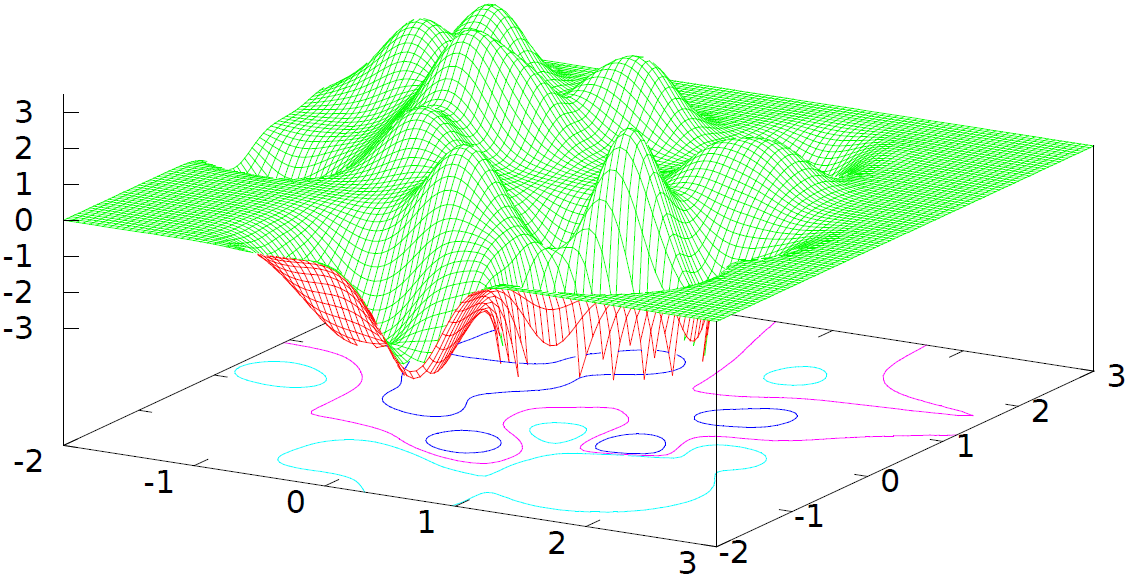
\includegraphics[height=10cm]{ml}

\vspace{\baselineskip}

In existing scientific literature, machine learning based predictive models for geomagnetic indexes can be classified as follows.

\begin{itemize}
    \item Non-linear auto-regressive
    \item Neural Network based
    \item Bayesian inference
\end{itemize}


\mysection{Gaussian Process Regression}

\vspace{\baselineskip}

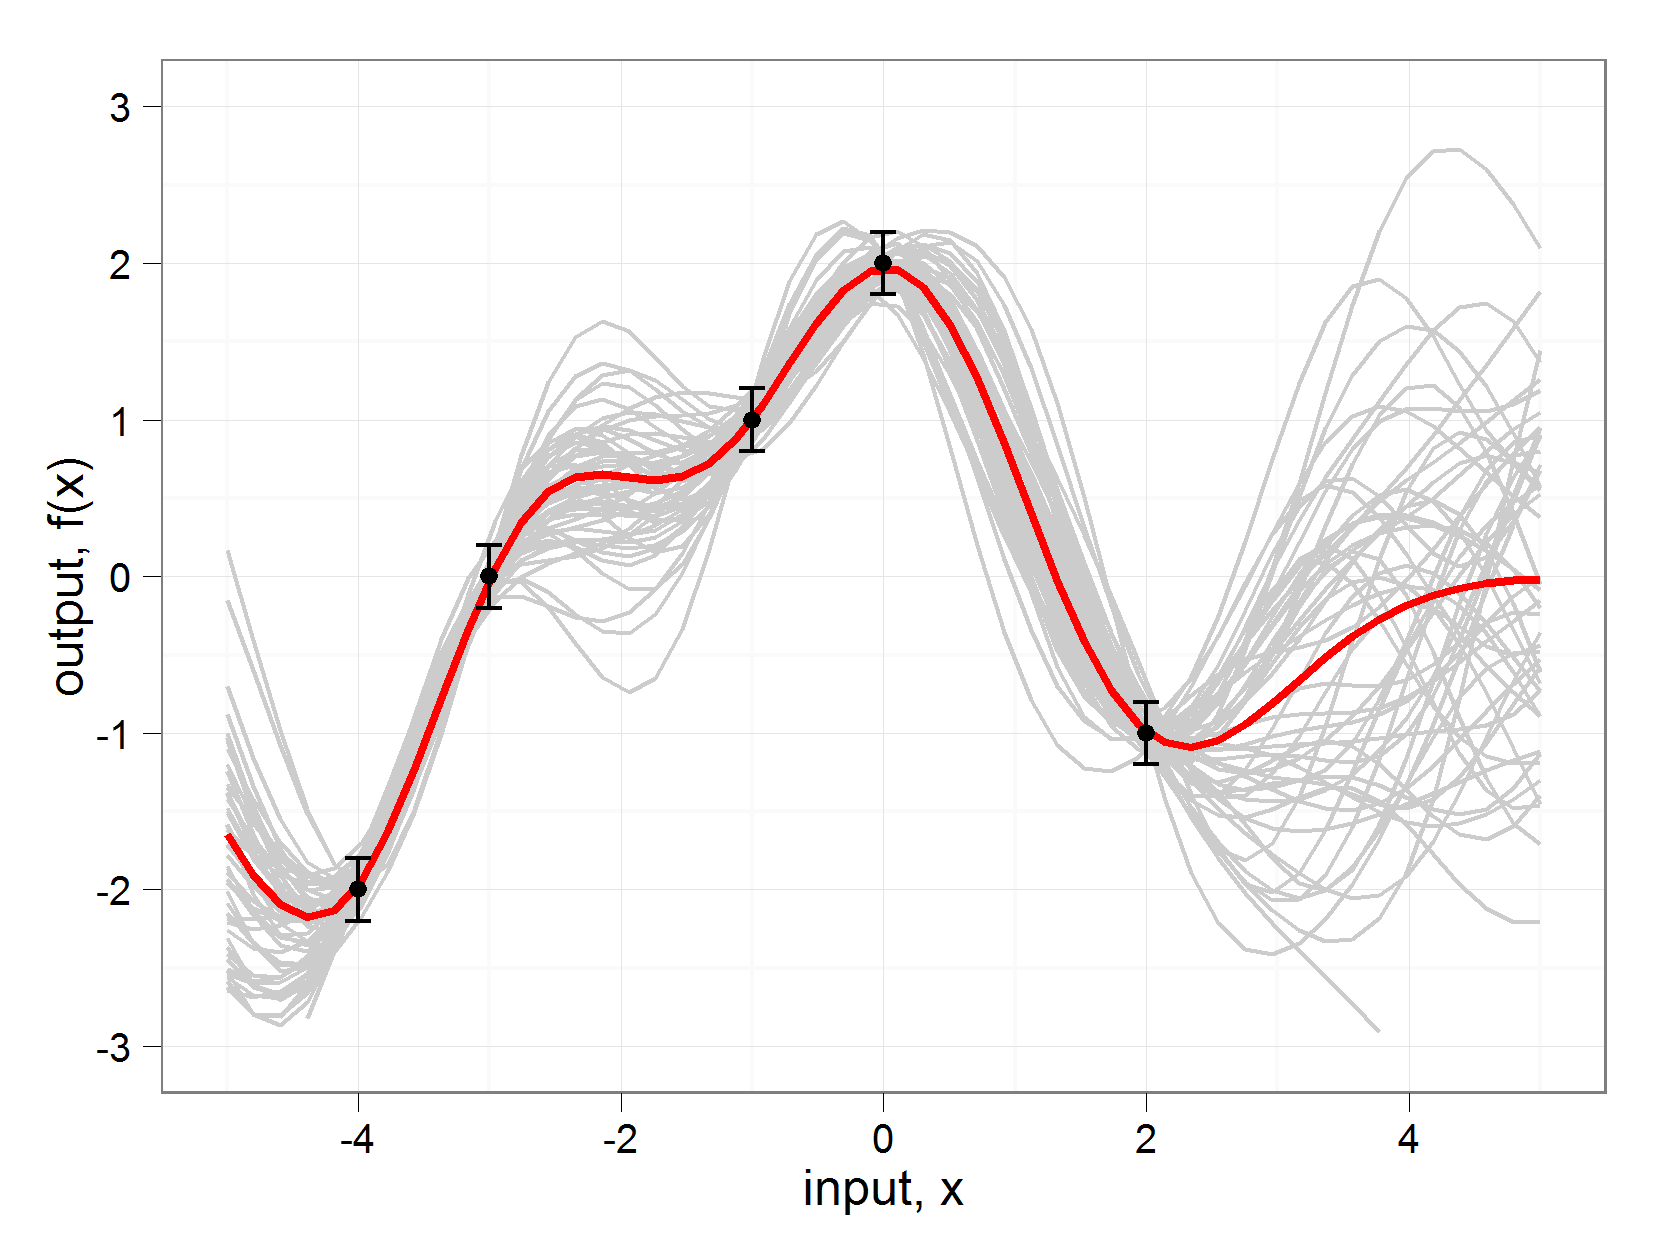
\includegraphics[height=10cm]{gp}

\vspace{\baselineskip}
 
 Gaussian Process models specify statistical distributions over functions, which can be designed by choosing appropriate covariance structures to model data. Estimates produced by such models are non-parametric in nature and are akin to fitting smoothing splines to data points.


\mysection{Predicting Dst using Gaussian Process driven by Fractional Brownian Covariance}

\vspace{\baselineskip}

Using the solar wind speed as a predictive variable, we propose a Gaussian Process model to predict the Dst index. For this purpose we propose to use the fractional Brownian covariance function to model the correlation between Dst values at different solar wind velocities $u$ and $v$.   

\vspace{\baselineskip}

$C(u,v) = |u|^{2H} + |v|^{2H} - |u-v|^{2H}$

\vspace{\baselineskip}

The parameter $H \ \in (0,1]$ called the Hurst parameter of the fractional Brownian kernel.

\begin{tabular}{ll}
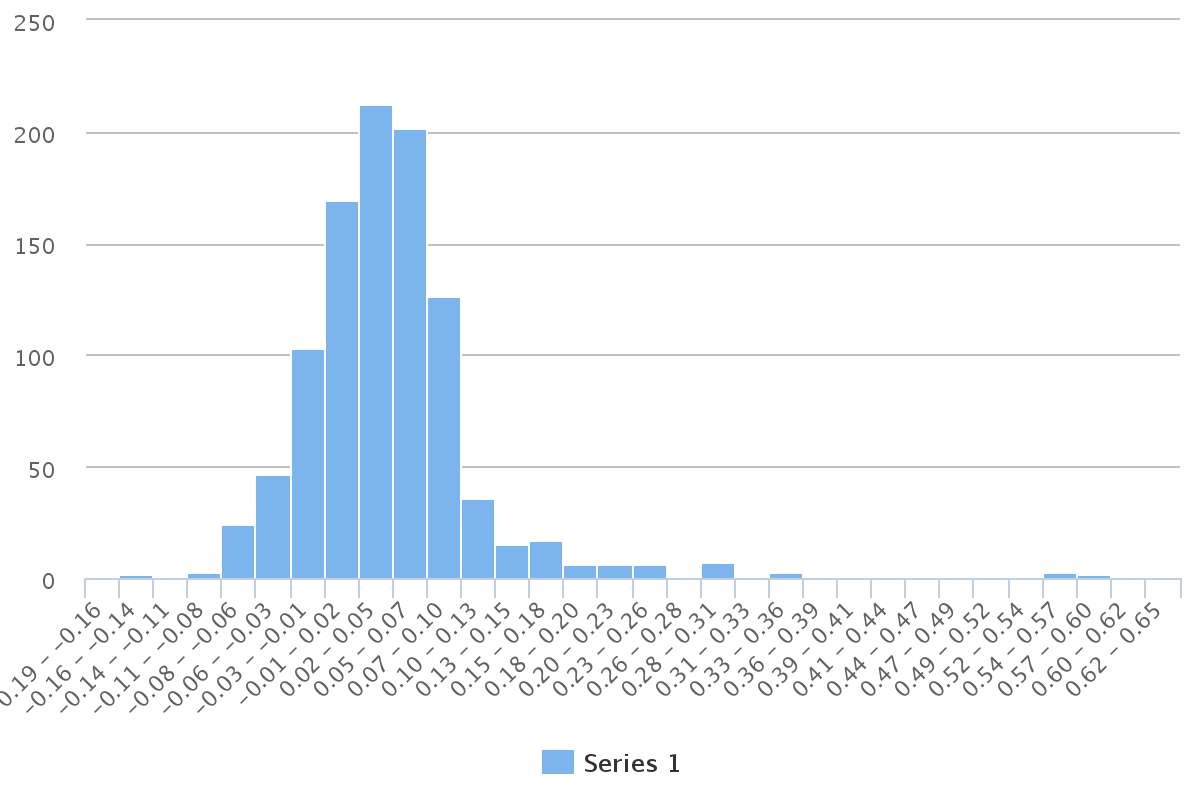
\includegraphics[height=10cm]{fit-hist}
&
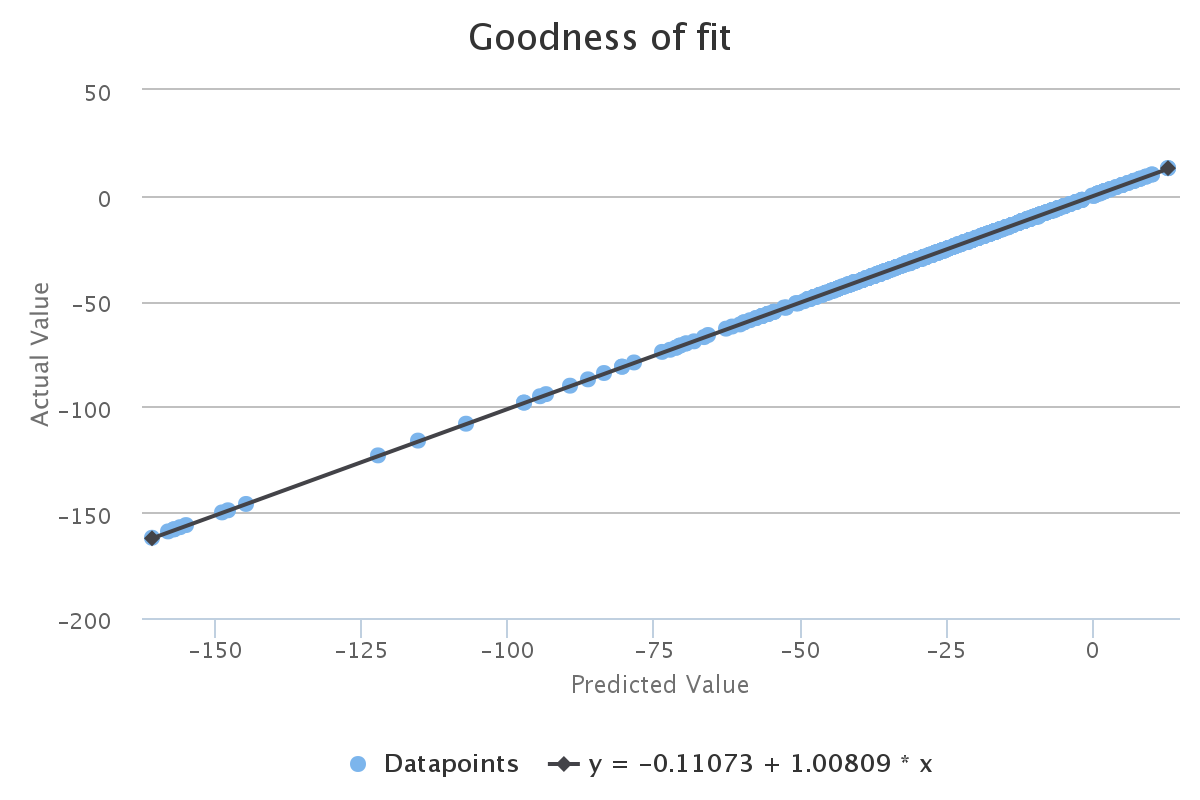
\includegraphics[height=10cm]{fit}
\end{tabular}
\caption{Left:}
\label{Fig:Race}

\end{multicols}

\end{poster}

\end{document}
